\chapter{Lezione 9}
Abbiamo visto fino ad ora distribuzioni di cariche elettriche nel vuoto, ora vediamo cosa succede all'interno di un materiale. Studieremo quindi i conduttori, dove le carice elettriche sono libere di muoversi, e gli isolanti/dielettrici, dove le cariche elettriche non sono libere di muoversi.

\section{Campo elettrico nei conduttori}
Lo studieremo nel caso di condizioni di equilibrio, cioè quando le cariche sono ferme. Dentro un conduttore il campo elettrico è nullo. Per vederlo utilizziamo la proprietà di conservazione del campo elettrico, in particolare utilizziamo il fatto che la circuitazione con cui calcoliamo il lavoro è zero, e utilizzeremo la legge di Gass che ci dice che il flusso del campo elettrico in una superficie chiusa è data da:
$$ \Phi_{\vec{E}}= \int_{S}^{} \vec{E}\cdot \vec{n} dS = 4\pi k_e Q_{int}$$

\begin{esempio}	
Consideriamo un corpo conduttore pieno che è carico elettricamente.Supponiamo di avere su di esso una carica negativa, ci chiediamo dove si trova. Poiche le cariche elettriche si possono muovere queste sono tutte di segno opposto allora si respingono una dall'altra e quindi raggiungono la superficie del conduttore. Uso il teorema di Gauss per ottenere che:
\begin{figure}[h]
	\begin{center}
		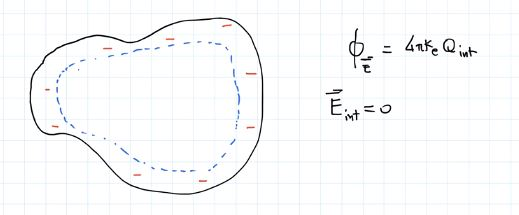
\includegraphics[width=8cm]{lezione9/images/1 Campo elettrico nei materiali.jpg}\\
		\caption{Campo in un conduttore carico}
	\end{center}
\end{figure}
\end{esempio}
\begin{esempio}
	
Consideriamo ora un corpo conduttore neutro posto all'interno di un campo elettrico. In questo caso se consideriamo una situazione di equilibrio troviamo che il campo all'interno è zero all'equilibrio, perchè le cariche elettriche che si muovevano sono ferme, se ci fosse ancora campo elettrico le cariche ne risentirebbero e continuerebbero a muoversi. Allora le cariche sono ferme se il campo elettrico interno è nullo. Usiamo il teorema di Gauss per capire come le cariche si distribuiscono:

\begin{figure}[h]
	\begin{center}
		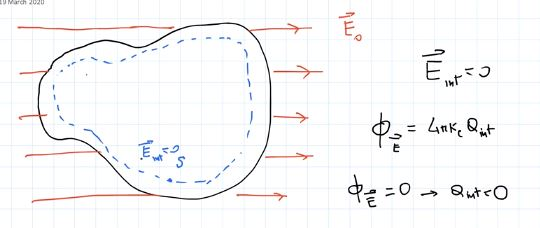
\includegraphics[width=8cm]{lezione9/images/2 Campo elettrico nei materiali.jpg}\\
		\caption{Campo in un conduttore non carico immerso in un campo.}
	\end{center}
\end{figure}

Esse si distribuiscono al bordo del conduttore poichè il disegno è valido per ogni superficie interna fino al bordo.
\end{esempio}

\begin{esempio}
	Consideriamo un conduttore cavo, e cerchiamo di capire quanto vale il campo elettrico all'interno della cavità. Sarà sempre valido che all'interno del conduttore ovunque il campo elettrico è comunque nullo. Se non fosse nullo avremmo una situazione del genere, che è assurda perchè il campo elettrico è conservativo.
	\begin{figure}[h]
		\begin{center}
			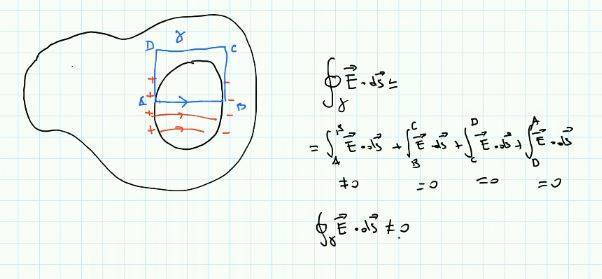
\includegraphics[width=8cm]{lezione9/images/3 Campo elettrico nei materiali.jpg}\\
			\caption{Campo elettrico in un conduttore cavo}
		\end{center}
	\end{figure}

Quindi il campo elettrico nel conduttore è zero, allora in generale il potenziale interno al conduttore è nullo poiche deve valere che $dV=-\vec{E} \cdot d\vec{s}$. Ma se noi introduciamo nella cavità una carica $q$, allora le cariche nel conduttore cominciano a muoversi accumulandosi vicino la cavità, e quindi si genera un campo elettrico nella cavità, e quindi in questi punti c'è una differenza di potenziale elettrico.

	\begin{figure}[h]
	\begin{center}
		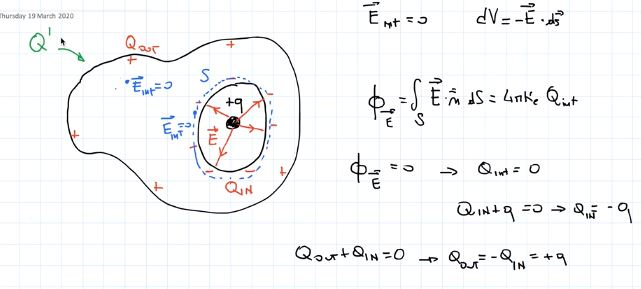
\includegraphics[width=10cm]{lezione9/images/4 Campo elettrico nei materiali.jpg}\\
		\caption{Gabbia di Faraday}
	\end{center}
\end{figure}

\end{esempio}


All'interno di un conduttore quindi il campo elettrico è nullo ma abbiamo della carica depositata sulla superficie del conduttore, allora ci chiediamo quanto vale il campo generato da essa in prossimità della superficie. Questo sarà certamente perpendicolare alla superficie, poichè altrimenti metterebbe in movimento le cariche violando l'equilibrio. Allora studiamo la situazione così:
	\begin{figure}[h]
	\begin{center}
		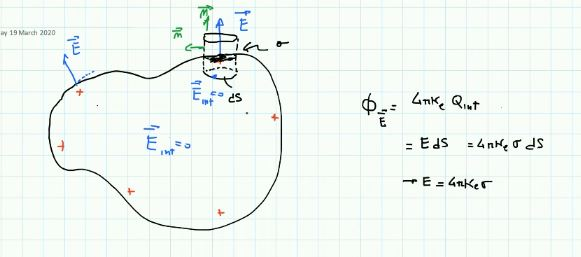
\includegraphics[width=10cm]{lezione9/images/5 Campo elettrico nei materiali.jpg}\\
		\caption{Campo elettrico sul bordo esterno di un conduttore}
	\end{center}
\end{figure}
\clearpage
\begin{esempio}(Forza delle punte)
	\begin{figure}[h]
	\begin{center}
		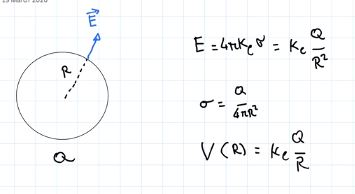
\includegraphics[width=6cm]{lezione9/images/6 Campo elettrico nei materiali.jpg}\\
		\caption{Potenziale di una sfera}
	\end{center}
\end{figure}
	\begin{figure}[h]
	\begin{center}
		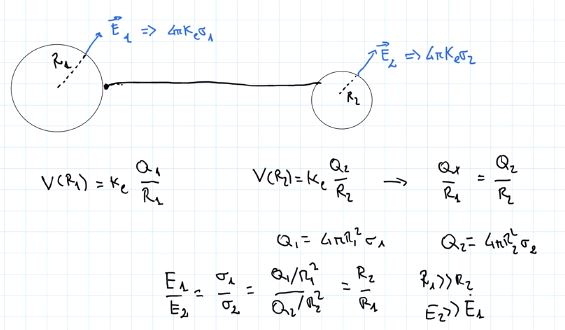
\includegraphics[width=6cm]{lezione9/images/7 Campo elettrico nei materiali.jpg}\\
		\caption{Potenziale di due sfere unite da un filo conduttore}
	\end{center}
\end{figure}

\end{esempio}

Cosa capita all'interno di un materiale isolante/dielettrico? cioè non ci sono portatori di carica liberi di muoversi. 
	\begin{figure}[h]
	\begin{center}
		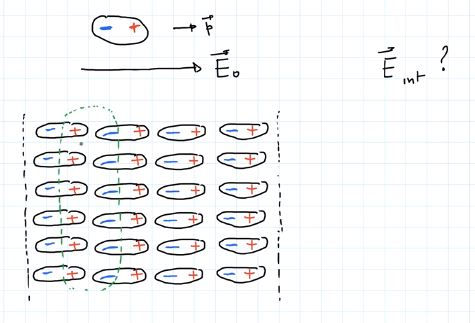
\includegraphics[width=6cm]{lezione9/images/8 Campo elettrico nei materiali.jpg}\\
		\caption{Campo nel caso di materiali isolanti}
	\end{center}
\end{figure}
	\begin{figure}[h]
	\begin{center}
		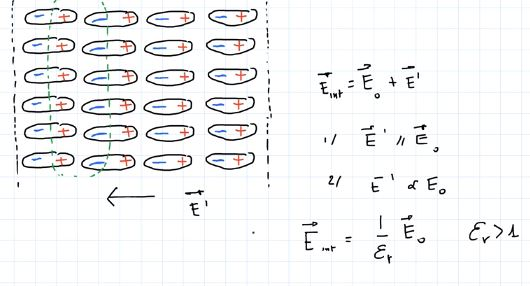
\includegraphics[width=6cm]{lezione9/images/9 Campo elettrico nei materiali.jpg}\\
		\caption{Gabbia di Faraday}
	\end{center}
\end{figure}